\subsection{Technological Background [ASH]}
The Smart Fridge leverages various existing technologies, new and old, in order to create a novel product.
All the underlying technologies such as the sensors used, the barcode detection and object detection already exists, and have seen usage in commercial settings such as with Amazon Fresh Stores \cite{fresh},
which allow shoppers to grab items and leave without having to manually scan them.
Bringing this technology into the home however represents a new market,
one which major companies such as Samsung \cite{samsung} are only now beginning to enter this market.
The Smart Fridge works towards pushing down the prices of these technologies by leveraging free and open-source technologies.

\subsection{Sustainability}

\subsubsection{Social [IP]}

One of the long run aims of the Smart Fridge is to reduce food waste by encouraging users to follow habits such as meal planning and consideration of the needless waste of products.
Food waste is one of the key contributing factors to world hunger.
Zero hunger is one of the seventeen UN Sustainable Development Goals \cite{UNGoals}.
Growing inequalities is one of the main factors to the undermining of food security worldwide.
Through efforts in trying to reduce food waste, world hunger can be significantly reduced.
Food waste can be broken down in different stages such as harvesting, storage and handling, processing, distribution, retail, and households.
Households have a contribution of approximately 40-50\% of total food waste \cite{FoodWasteStages}, which is the largest portion comparing to the rest of the stages of food waste.
There are various reasons behind food waste in households, such as lack of meal planning, and consideration.
A very common scenario is poor planning which occurs when people buy products from the supermarket with the aim of making a specific recipe but also without having a recipe in mind.
In either case, the products might end not being used before their expiration date and hence wasted.
Overbuying is another very common case, where people buy products without considering products that they already have and end up not being able to use them all before their expiration date.

Another issue that many people face is having poor nutrition, neglecting the importance of eating healthy and nutritious foods.
Tracking the products contained in the user's fridge and recommending healthy recipes suggestions, a healthier lifestyle is promoted.
With a Smart Fridge the user can focus on their nutritional needs, which is not very common nowadays.
Additionally, it will be possible to track from anywhere what products they already have and so be reminded of what they own and how they can use it.
Knowing what products, they have allows people to put into consideration what they want to cook, hence be more open to spending time cooking more nutritionally rich foods.
This can be extended to meal planning, depending on the commitment of the user.

\subsubsection{Economic [JG, IP]}

The users can track their products from anywhere using the product's website, while checking what they need to buy when shopping in case they haven't done so before.
The Smart Fridge's inventory records the products using two features, barcode scanning and object recognition.
The inventory can prevent users not only from buying products that they might already have, but also consider using the ones they have before buying new ones.
Therefore, grocery shopping can be done more sustainably, while also saving money.
Another aspect of checking the groceries inside the fridge to consider, is that people tend to open and close the fridge door too often, also leaving it open for long.
This increases the power consumption of the fridge, and so being able to check what is inside the fridge without the need to open and close the door multiple times, the power usage can be decreased, as well as the energy bills of the household.

According to \cite{bandoim_2020}, the average American household wastes somewhere between 30 to 40\% of their food, which amounts to over \$1800 worth of food wasted per household annually or \$240 billion in total.
Therefore, one of the goals set out with the Smart Fridge was to design a product that would help households reduce the amount of food they waste.
Each feature of the Smart Fridge was implemented with this goal in mind.

However, \cite{bandoim_2020} also states that, despite households that used shopping lists wasting less food, even the most frugal household wasted nearly 10\% of their food.
The study conducted in \cite{bandoim_2020} concluded that one of the leading reasons for food waste was food spoiling before the household had the chance to eat it.
Therefore, the Smart Fridge can automatically detect expiration dates on products, and remind the user about upcoming expiration dates.

\subsubsection{Environmental [IP]} 
Preventing food waste can alleviate the negative impact it has on the environment.
Most people that overbuy and don't meal plan end up wasting a lot of the products they have bought as these products have either expired and cannot be used.
All food waste can have a significant contribution to global warming.
Food waste breaks down in landfills and decomposes into methane that is released in the atmosphere.
Methane is one of the key greenhouse gases contributing to global warming \cite{foodwaste}.
Therefore, having a system that allows tracking and reducing the waste of products, can have a positive effect in the minimisation of food waste.
Additionally, as forementioned the tracking of products through a website, can reduce the power usage of the fridge as the user minimises the time, they have the fridge door open.
The UN Sustainability Goals aimed to be approached through the Smart Fridge are the following:

\begin{itemize}
    \item Goal 2 - Zero Hunger
    \item Goal 3 - Good Health and Well-being
    \item Goal 8 - Decent 	Work and Economic Growth
    \item Goal 12 - Responsible Consumption and Production
   \item Goal 13 - Climate Action 
\end{itemize}

\subsubsection{Circular Economy [HH]}

A circular economy is an economic system that is restorative and "regenerative by design" \cite{circ}.
In a circular economy, resources are kept in use for as long as possible, and after they are no longer useful, they are recovered
and regenerated into new products or materials.
This is contrasts radically to the traditional linear economy, in which resources are continuously extracted, used,
and then discarded as waste.
In a circular economy, waste is minimised, resources are used efficiently, the global economy develops sustainably, and the planet ceases to be recklessly exploited.

The Smart Fridge is designed with the principles of a circular economy in mind, maximizing resource efficiency and minimizing waste.

The use of open-source designs such as the Raspberry Pi and ESP32 contribute to this goal.
These microcontrollers and single-board computers are open-source, meaning that their hardware and software can be freely accessed and modified by anyone.
This allows for easy repairs and replacements, as well as the ability to upgrade the hardware.
The open-source nature of these components also makes the manufacturing process more efficient because accessibility and collaboration reduce the cost of research development and accelerates innovation.
The goal is to make the most optimal product, in contrast with the linear economy's obsession with planned obsolescence, designed to maximise consumption and spending.

In addition to being open source, the Smart Fridge is designed with strong and reliable components, as well as scratch-resistant acrylic, all of which contribute to its extended lifetime of over 10 years.
These design elements, along with the ability to easily disassemble and reassemble the fridge for repairs, make it a sustainable and cost-effective choice.

Annually, opening the fridge door can increase energy consumption by 120kWh \cite{energy}.
When the door is opened, cold air escapes and is replaced with warm air.
Consequently, the cooling systems must work harder to maintain the colder optimal temperature.
By using the Smart Fridge, the inventory can be viewed without opening the door significantly limiting the cold air that can escape.
A side effect is that since the cooling systems are less burdened, they will have an extended lifetime.
And while the Smart Fridge features extra electronic components such as cameras, these are on standby until activated by the Hall sensor.
Moreover, the energy that the Smart system saves vastly outweighs its relatively negligible power consumption.
Therefore using the Smart Fridge's inventory management capabilities can significantly reduce energy usage by reducing the burden on the cooling system.

The Smart Fridge is designed with repairability and upgradeability in mind, with the goal of extending its lifetime.
Key components such as the ESP32, camera,  and Raspberry Pi can easily be replaced if needed, thanks to their connection via cables or headers rather than being directly soldered onto the stripboard.
This makes it easy to remove and examine components for repairs or replacements.
It's possible to replace components with stronger counterparts; if a consumer desires enhanced visual fidelity or a wider viewing angle, the camera can easily be replaced.

When a product reaches the end of its life, recoverability is paramount.
Fortunately, the use of screws rather than glue to secure hinges and panels also makes it easy to disassemble (and reassemble) the fridge.
Also, the fridge's refrigeration components and smart electronic hardware are physically isolated from each other, allowing for safe extraction of the electronic components.
This helps to minimize waste and promote sustainability.

\subsection{System Overview [IB]}
The objective of the overall system is to autonomously track the inventory of a fridge.
Our approach to solve this objective was to split the system into several sub systems.
There are 4 components connected to the ESP32 microcontroller: the HX711 load cell measures the weight of the contents of the fridge and needs between 3.3V and 5V to operate, a HAL sensor requires 2.8-6V of power and is used to detect weather the fridge door is open, a 5V LED strip to light up the fridge and a buzzer that sounds when the fridge has been open too long.
The direction of the item is quantified by calculating the change in weight.
This value is packaged in a JSON packet with the ON/OFF state of the fridge door and the alarm state and sent to the Raspberry Pi via UART serial communication.
The hardware is powered by a 9V barrel jack and is stepped down by a switch mode power supply to 3.3V and 5V.
A 5V USB web camera is connected to the PI and captures the item as it enters the fridge.
OpenCV is used to detect what item is entering the fridge.
The inventory information and the direction are then sent to a PostgreSQL database using GraphQL communication.
Depending on the item's direction, the item will be added or removed from the database.
This database acts as a backend for the products website/app.

\begin{figure}[H]        
    \centering
    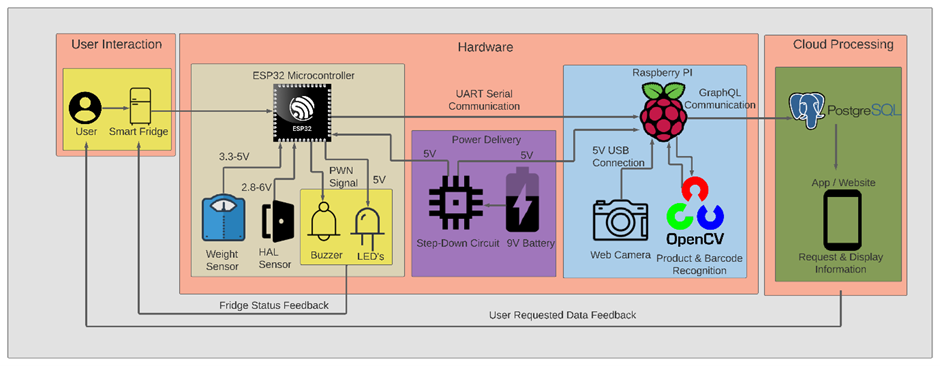
\includegraphics[width=1\textwidth]{Chapter 2/SystemOverview.png}
    \caption{System Overview Block Diagram}
    \label{fig:blockdia}
\end{figure} 

The project can be split into 3 main groups: the microprocessor group who will design the hardware which will collect the data, the Raspberry Pi group who will use OpenCV to detect the item and the cloud processing team who will deal with the server and website side of the design.
Within each group the tasks can be split between each member.
For example, in the microprocessor team, each member can be assigned to a different component and in the cloud processing team one member can focus on the front-end design and the other on the back end.
By splitting the project into smaller objectives, work can be completed independently and in parallel and the number dependencies between members can be reduced.
This will make the project run much more efficiently.
The individual teams will however need to communicate when planning on how to integrate the work together.
The sub systems and their dependencies have been outlined in table %\ref{tab:depend}.

\subsection{Dependency Table [IB]}
% Please add the following required packages to your document preamble:
% \usepackage{longtable}
% Note: It may be necessary to compile the document several times to get a multi-page table to line up properly
\begin{longtable}[c]{|l|l|l|}
  \caption{Dependency Table}
  \label{tab:depend}\\
  \hline
  \textbf{Sub-System} &
    \textbf{Sub-System Aims} &
    \textbf{Dependency} \\ \hline
  \endfirsthead
  %
  \endhead
  %
  \begin{tabular}[c]{@{}l@{}}HX711 Load Cell\\ Weight Sensor\end{tabular} &
    \begin{tabular}[c]{@{}l@{}}The Weight Sensor measures\\ the weight of all items placed\\ on top of it. The value is sent\\ to the ESP32.\end{tabular} &
    \begin{tabular}[c]{@{}l@{}}Needs between 3.3V\\ and 5V to operate.\end{tabular} \\ \hline
  HAL Sensor &
    \begin{tabular}[c]{@{}l@{}}Sends an ON/OFF state to the\\ ESP32 when the fridge door\\ is open.\end{tabular} &
    \begin{tabular}[c]{@{}l@{}}Needs between 2.8V\\ and 6V to operate.\end{tabular} \\ \hline
  Piezo Buzzer &
    \begin{tabular}[c]{@{}l@{}}When the doors been open\\ after a limit, the buzzer will\\ sound.\end{tabular} &
    \begin{tabular}[c]{@{}l@{}}The ESP32 sends a\\ square PWN signal to\\ the buzzer. The\\ frequency is set by\\ the ESP32 code.\end{tabular} \\ \hline
  LED’s &
    \begin{tabular}[c]{@{}l@{}}Lights the fridge when it\\ opens.\end{tabular} &
    \begin{tabular}[c]{@{}l@{}}Needs between 5V\\ to operate.\end{tabular} \\ \hline
  ESP32 Microprocessor &
    \begin{tabular}[c]{@{}l@{}}Controls the operation of\\ the sensors for the fridge.\\ Packets the sensor data in a\\ JSON packet which is sent to\\ the Raspberry PI. Needs to\\ calculate the direction of the\\ item using the change in\\ weight value.\end{tabular} &
    \begin{tabular}[c]{@{}l@{}}Needs 5V power from\\ the step-down circuit\\ built on the PCB. \\ Requires weight value\\ from the weight sensor\\ and the ON/OFF state\\ from the HAL sensor.\end{tabular} \\ \hline
  Raspberry PI &
    \begin{tabular}[c]{@{}l@{}}Uses web camera image and\\ OpenCV to detect the items\\ entering the fridge. Sends the\\ inventory data to the cloud\\ database using GraphQL\\ communication.\end{tabular} &
    \begin{tabular}[c]{@{}l@{}}Needs 5V power from\\ the step-down circuit\\ built on the PCB. Requires\\ web camera image of\\ inside the fridge. Requires\\ JSON packet containing \\ item direction, ON/OFF \\ state from the HAL sensor\\ and alarm state. This is \\ sent via UART using \\ Serial communication.\end{tabular} \\ \hline
  Web Camera &
    \begin{tabular}[c]{@{}l@{}}Captures images of the\\ product as it enters and exits\\ the fridge.\end{tabular} &
    \begin{tabular}[c]{@{}l@{}}5V power connected\\ via USB from the\\ Raspberry PI.\end{tabular} \\ \hline
  PostgreSQL &
    \begin{tabular}[c]{@{}l@{}}Stores the inventory data\\ sent from the Raspberry PI.\end{tabular} &
    \begin{tabular}[c]{@{}l@{}}Receives the inventory\\ data from the Raspberry\\ PI via GraphQL communication.\end{tabular} \\ \hline
  \end{longtable}

\subsection{MOSCOW Diagram [IB]}
% Please add the following required packages to your document preamble:
% \usepackage{longtable}
% Note: It may be necessary to compile the document several times to get a multi-page table to line up properly
\small
\begin{longtable}[c]{|l|l|l|}
    \caption{Moscow}
    \label{tab:moscow }\\
    \hline
    \textbf{Must Have}                         & \textbf{Should Have}                                                                            & \textbf{Could Have}        \\ \hline
    \endfirsthead
    %
    \endhead
    %
    \begin{tabular}[c]{@{}l@{}}A Camera to film products \\ entering the fridge.\end{tabular} &
      \begin{tabular}[c]{@{}l@{}}Weight sensor to detect if an item \\ is entering or leaving the box.\end{tabular} &
      \begin{tabular}[c]{@{}l@{}}LEDs to light up the \\ inside of the fridge.\end{tabular} \\ \hline
    \begin{tabular}[c]{@{}l@{}}Transmission from the \\ hardware to the server.\end{tabular} &
      \begin{tabular}[c]{@{}l@{}}Hal sensor to trigger turning \\ the camera on.\end{tabular} &
      An alarm to signal that the \\ fridge has been open too long. \\ \hline
    Inventory data displayed on a website/app. & \begin{tabular}[c]{@{}l@{}}A prototype fridge to enclose \\ the hardware.\end{tabular}          & Expiration date detection. \\ \hline
    Barcode detection program.                 & Object detection.                                                                               &                            \\ \hline
                                               & \begin{tabular}[c]{@{}l@{}}Display recipes on the website \\ using inventory data.\end{tabular} &                            \\ \hline
    \end{longtable}

\subsection{SWOT Analysis [IB]}
% Please add the following required packages to your document preamble:
% \usepackage{longtable}
% Note: It may be necessary to compile the document several times to get a multi-page table to line up properly
\begin{longtable}[c]{|l|l|}
    \caption{SWOT Analysis}
    \label{tab:swot}\\
    \hline
    \begin{tabular}[c]{@{}l@{}}Strengths:\\    \\ - Helps the user  keep track of the \\ products in their  fridge and therefore\\ helps reduce waste.\\ - Helping the  user not buy unnecessary\\ food, which will save them money and \\ make   investing in the product worth it.  \\ - The app  promotes healthy diets which\\ will help the user live a healthier life.\\ - Similar   products require the user to\\ change their daily routine to operate. Our \\ Product is autonomous and doesn't require\\ the user to do anything.\\ - Given that the  prototype can be produced\\ for under £100, the additional price increase\\ compared to a  normal fridge is relatively low.\end{tabular} &
      \begin{tabular}[c]{@{}l@{}}Weakness:\\    \\ - Item detection needs to be very accurate \\ so that user doesn't need to manually\\ enter the items.\\ - Similar looking items might confuse the \\ computer vision system.\\ - The product requires the user to own a\\ and want to use smart phone, this might\\ reduce the pool of customers.\end{tabular} \\ \hline
    \endfirsthead
    %
    \endhead
    %
    \begin{tabular}[c]{@{}l@{}}Opportunities:\\  \\ - There are very few similar products on\\ the market. \\ - Most households have fridges. When they\\ are replaced, users are looking for unique\\ selling features. This makes our product very\\ desirable. \\ - Could be sold globally.\end{tabular} &
      \begin{tabular}[c]{@{}l@{}}Threats:\\    \\ - The fridge market is very large therefore\\ it  would be difficult to make this product\\ stand out despite its unique selling feature.\\ - Patents would be required, otherwise \\ better funded companies could outperform \\ the Smart Fridge.\\ - Convincing customers to spend more\\ money on the product than a normal fridge\\ would mean that the benefits would need to\\ be very clear with strong marketing. This\\ would cost significant amounts of money.\end{tabular} \\ \hline
    \end{longtable}

\subsection{Client Requirements [IB]}
% Please add the following required packages to your document preamble:
% \usepackage{longtable}
% Note: It may be necessary to compile the document several times to get a multi-page table to line up properly
\small
\begin{longtable}[c]{|l|l|l|}
  \caption{Client Requirements }
  \label{tab:clientreq}\\
  \hline
  Client  Requirement &
    \begin{tabular}[c]{@{}l@{}}Description  Of Product \\ Implementation\end{tabular} &
    \begin{tabular}[c]{@{}l@{}}Has The Requirement  \\ Been Met?\end{tabular} \\ \hline
  \endfirsthead
  %
  \endhead
  %
  \begin{tabular}[c]{@{}l@{}}There must be an aspect of hardware\\  associated with data generation,\\ measurement, and recording.\end{tabular} &
    \begin{tabular}[c]{@{}l@{}}The HX711 Load cell measures the\\ weight, the HAL Sensor measures\\ the ON/OFF state and the web \\ camera which is connected to a\\ Raspberry PI detects the product \\ entering the fridge using OpenCV.\end{tabular} &
    Yes \\ \hline
  \begin{tabular}[c]{@{}l@{}}There  must be an aspect of timed \\ data transmission to a known free\\ secure location.\end{tabular} &
    \begin{tabular}[c]{@{}l@{}}Supabase and it's API is used to\\ send data to and from the PI, \\ Website and App to a PostgreSQL\\ database.\end{tabular} &
    Yes \\ \hline
  \begin{tabular}[c]{@{}l@{}}There must be an aspect of timed\\ data  display and analysis on a\\ portable device.\end{tabular} &
    \begin{tabular}[c]{@{}l@{}}The Inventory Data is displayed\\ on a  website and an App which\\ can be view on a portable device.\end{tabular} &
    Yes \\ \hline
  \begin{tabular}[c]{@{}l@{}}There  must be documentation\\ with evidence of testing and\\ validation.\end{tabular} &
    \begin{tabular}[c]{@{}l@{}}This  document contains all the\\ evidence of testing and validation\\ throughout this project.\end{tabular} &
    Yes \\ \hline
  \begin{tabular}[c]{@{}l@{}}The cost of the project must not\\ exceed  £100.\end{tabular} &
    \begin{tabular}[c]{@{}l@{}}The cost of the project was kept\\ below  £100.\end{tabular} &
    Yes \\ \hline
  \end{longtable}


\subsection{Phase Diagram [IB]}

\begin{figure}[H]        
    \centering
    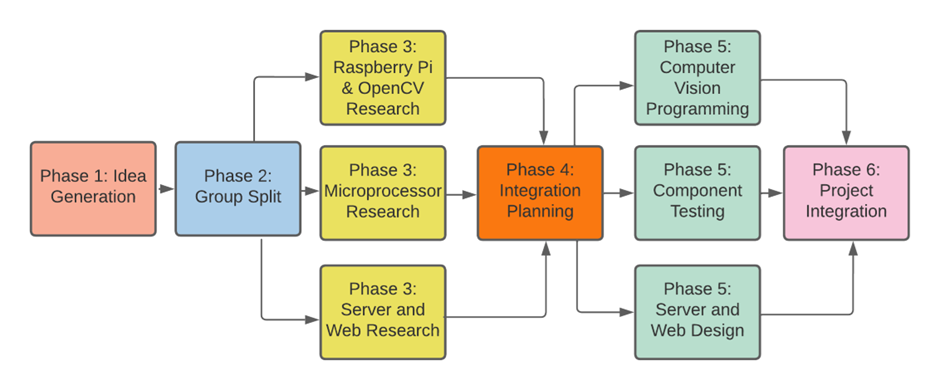
\includegraphics[width=1\textwidth]{Chapter 2/PhaseDiagram.png}
    \caption{Phase Diagram}
    \label{fig:phasediag}
\end{figure} 

The first phase of the project was to generate ideas for the project which followed the specification and vote on which idea to put forward.
Phase 2 is when the group discusses the individual members strengths and weaknesses and decides who is best suited to each team.
Phase 3 is the research phase, and it involves looking into what software and components could be used whilst considering their feasibility.

At the end of this phase a plan should be formed to start designing and testing the tasks of each group as well as ordering the required parts.
Phase 4 is aimed at coming together as a group and forming a plan to integrate the individual teams work together.
This includes discussions of dependencies that each sub team have on each other.
Phase 5 is when the individual teams build and test their work and phase 6 is when the work of the 3 teams is integrated together.